\hypertarget{P135}{}
\begin{solution}{normal} % 135
One method of measuring magnetic field is as follows. A small coil is inserted into the magnetic field with its axis parallel to $\textbf{\textit{B}}$. The terminals of the coil are connected to a ballistic galvanometer, which measures the amount of charge passed through it. The coil is then quickly rotated $180\degree$. How much charge passes through the galvanometer if the area of the coil is $S$, the number of turns is $N$, and the resistance of the coil is $R$?
\end{solution}

\hypertarget{P136}{}
\begin{solution}{normal} % 136
Two horizontal infinitely long parallel metal rails with negligible resistance are placed a distance $l$ from each other. The rails are connected to a capacitor of capacitance $C$ and voltage $U_0$. If there is a homogeneous vertical magnetic field of magnitude $\textbf{\textit{B}}$, a) what is the maximum velocity the rod reaches, and b) what is the maximum possible efficiency of such an "electromagnetic cannon" (i.e. how much of the energy stored in the capacitor can be converted into kinetic energy in the rod)?
\end{solution}

\hypertarget{P137}{}
\begin{solution}{normal} % 137
A dielectric ring of mass $m$ is attached by spokes of negligible mass to an axis around which it can rotate frictionlessly. A charge $Q$ is evenly distributed over the ring. Initially, the (stationary) ring is located along the axis of a homogeneous magnetic field $\textbf{\textit{B}}$. After some time, the magnetic field is switched off. What is the final angular velocity of the ring?
\end{solution}

\hypertarget{P138}{}
\begin{solution}{normal} % 138
In the circuit below, switch $K$ has been closed for a long time and all the bulbs have the same brightness. For each of the bulbs, how many times does the current through the bulb change immediately after opening switch $K$.
\begin{center}
    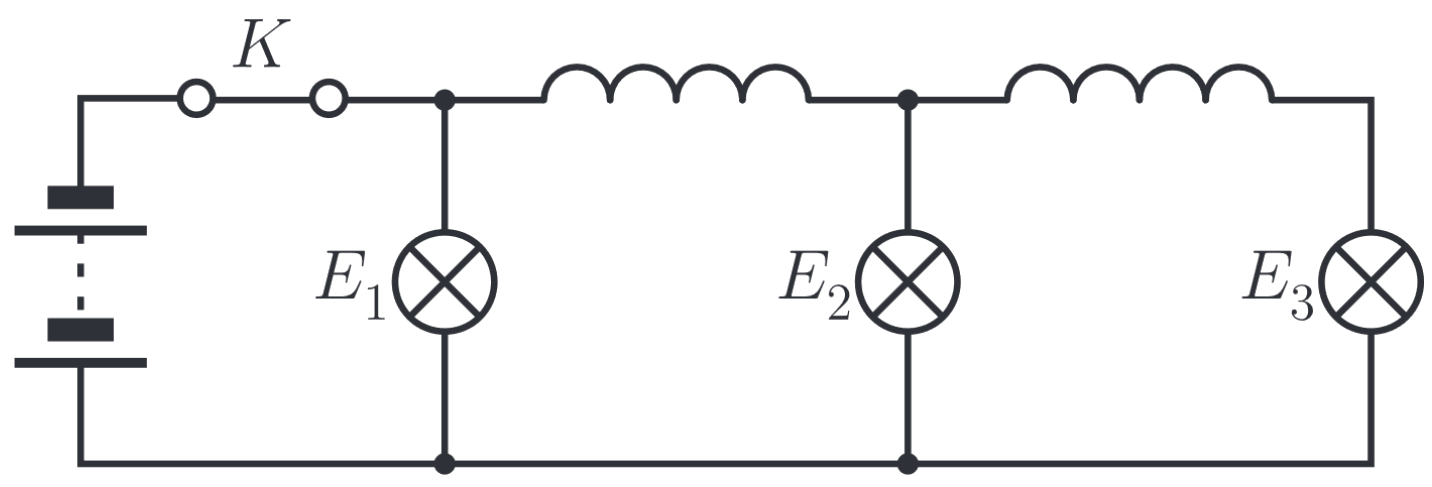
\includegraphics[width=0.8\textwidth]{S5 Figures/S5-138.png}
\end{center}
\end{solution}
\newpage
\hypertarget{P139}{}
\begin{solution}{normal} % 139
In the circuit shown below, switch $K$ has been open for a long time. a) What is the ammeter reading immediately after closing the switch? b) The switch is kept closed until the current reaches a steady state. What is the ammeter reading now? c) After the current has reached a steady state, what is the ammeter reading immediately after opening the switch?
\begin{center}
    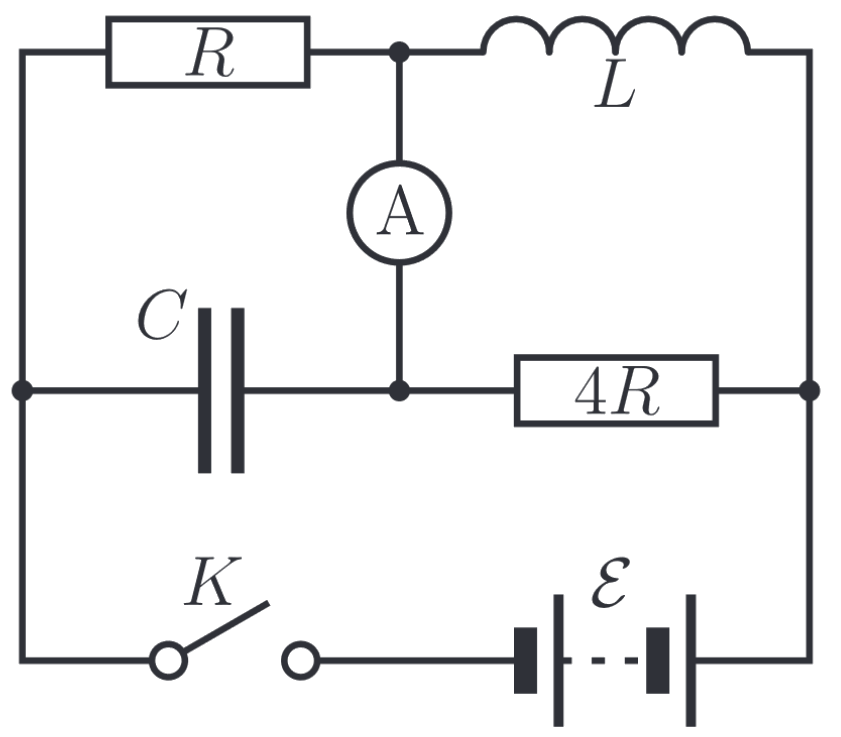
\includegraphics[width=0.4\textwidth]{S5 Figures/S5-139.png}
\end{center}
\end{solution}

\hypertarget{P140}{}
\begin{solution}{normal} % 140
Circuit element $E$ with $I-V$ dependence as shown in the graph below is connected to a circuit an inductor and battery. How does the voltage on element $E$ change over time? Determine time steps.
\begin{center}
    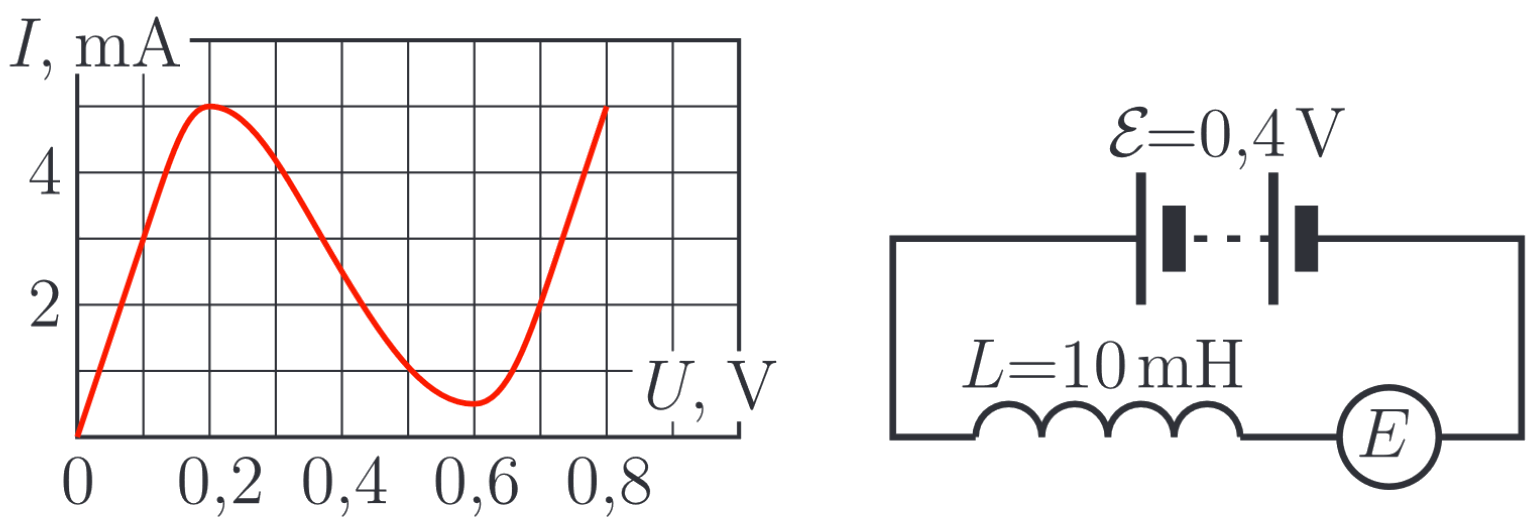
\includegraphics[width=0.8\textwidth]{S5 Figures/S5-140.png}
\end{center}
\end{solution}

\hypertarget{P141}{}
\begin{solution}{normal} % 141
A battery with emf $\mathcal{E}=12\;\text{V}$ is charged by a DC voltage source as shown in the figure below. The inductance in the coil is $L=1\;\text{H}$ and it has negligible resistance. The diode can be assumed to be ideal. Switch $K$ closes and opens periodically, alternating from being closed for time $\tau_1$ to being open for time $\tau_2$, where $\tau_1=\tau_2=0.01\;\text{s}$. Determine the average charging current.
\begin{center}
    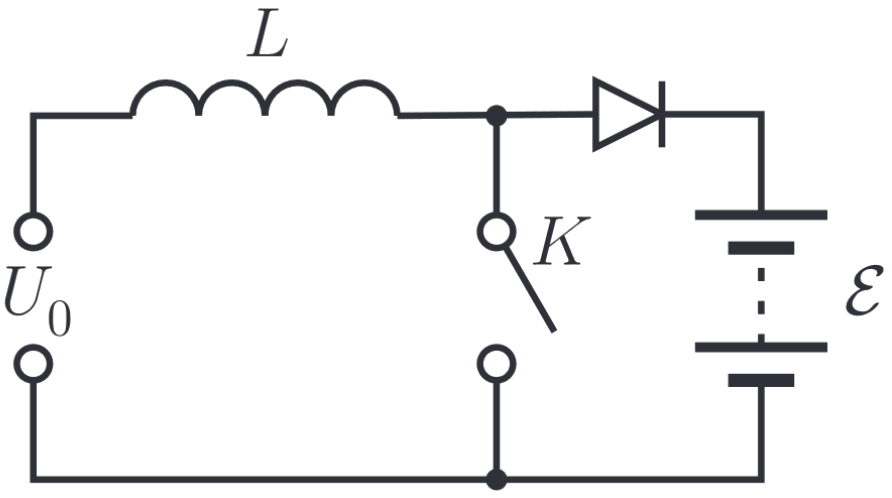
\includegraphics[width=0.45\textwidth]{S5 Figures/S5-141.png}
\end{center}
\end{solution}

\hypertarget{P142}{}
\begin{solution}{normal} % 142
Determine the inductance of a solenoid if its diameter is much smaller than its length $l$. The number of turns is $N$ and the cross-sectional area of the solenoid is $S$. The solenoid is wound around a ferromagnetic core with relative magnetic permeability $\mu$.
\end{solution}

\hypertarget{P143}{}
\begin{solution}{normal} % 143
Assuming that the work done to generate current in a solenoid $LI^2/2$ goes into the energy of its magnetic field, show that the energy density of the magnetic field is given by $B^2/2\mu_0$.
\end{solution}

\hypertarget{P144}{}
\begin{solution}{normal} % 144
Determine the inductance of a straight wire of length $l$ and radius $a$.
\end{solution}

\hypertarget{P145}{}
\begin{solution}{normal} % 145
Show that the mutual inductances $L_{12}$ and $L_{21}$ are always equal. \textit{Note:} Find the energy of the coupled circuits if the currents $I_1$ and $I_2$ flow through them. To do this, calculate the work the current sources need to do in order to generate the currents and show that the result is unambiguous only under the condition $L_{12}=L_{21}$.
\end{solution}

\hypertarget{P146}{}
\begin{solution}{normal} % 146
Show that $M\leq\sqrt{L_1L_2}$, where $M$ is the mutual inductance and $L_1,L_2$ are the self-inductances of the coupled circuits. \textit{Note:} Show that for $M>\sqrt{L_1L_2}$, conservation of energy is violated, namely that increasing the current in one of the circuits induces an emf in the circuit, which causes the current to increase further ($\mathcal{E}_1dI_1>0$).
\end{solution}

\hypertarget{P147}{}
\begin{solution}{normal} % 147
A toroid consists of a thin wire wrapped around a torus. Let the major and minor radii of the toroid be $R$ and $r$, respectively, where $r\ll R$ and let the number of turns of the wire be $N$. Determine the mutual inductance between the toroid and a straight wire. Prove that the equation $L_{12}=L_{21}$ is valid for this system.
\end{solution}

\hypertarget{P148}{}
\begin{solution}{normal} % 148
Determine the mutual inductance between two coils wrapped around a common toroidal core. The first coil has $N_1$ turns and the second has $N_2$ turns. The length of the core is $l$ and has cross-sectional area $S$ and relative magnetic permeability $\mu$.
\end{solution}

\hypertarget{P149}{}
\begin{solution}{normal} % 149
Two coils are wound around a common ferromagnetic core. The first has $N_1$ turns and the second $N_2$ turns, where $N_1/N_2=n$. The coils have negligible resistance. The ends of the second coil are connected to resistor $R$, and a DC voltage source of voltage $U$ is connected to the terminals of the first coil. Show that the power dissipated by the resistor is given by $n^2U^2/R$.
\end{solution}

\hypertarget{P150}{}
\begin{solution}{normal} % 150
A capacitor with capacitance $C$ is charged with an inductor and a diode from a constant voltage source $\mathcal{E}$. The internal resistance of the voltage source and the resistance of the coils are negligible. a) What was the voltage across the capacitor at the beginning when the charge on the capacitor was zero? b) What is the maximum current in the circuit? The $I-V$ graph of the diode is given in the graph below.
\begin{center}
    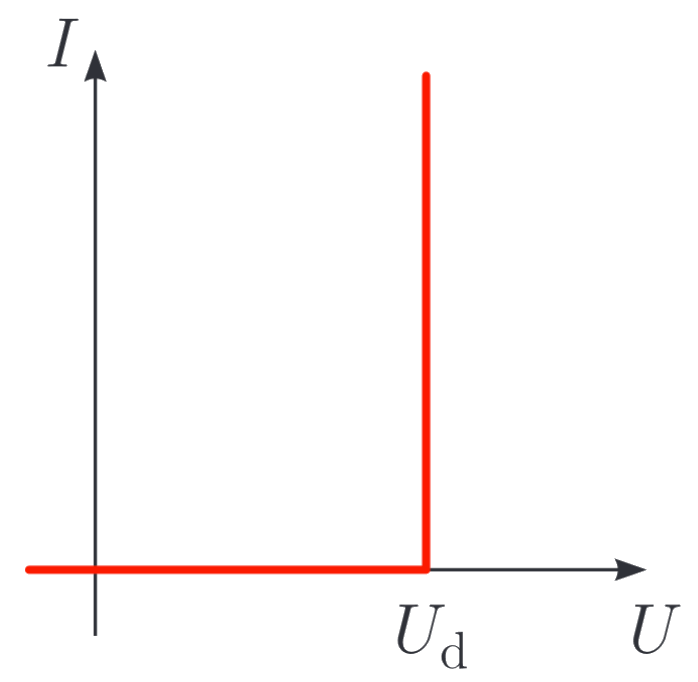
\includegraphics[width=0.4\textwidth]{S1 Figures/S1-35-2.png}
\end{center}
\end{solution}

\hypertarget{P151}{}
\begin{solution}{normal} % 151
In the circuit shown below, capacitors $C_1$ and $C_2$ are charged by a DC voltage source of emf $\mathcal{E}$. Switch $K$ is now closed. What is a) the maximum current $I_\text{max}$ through the coil, and b) the maximum voltage $U_\text{max}$ on capacitor $C_1$ achieved after closing the switch? \textit{Note:} To answer part b, note that if capacitor $C_1$ has maximal voltage across it then $C_2$ has minimal voltage across it as the sum of these voltages are constant (and equal to $\mathcal{E}$).
\begin{center}
    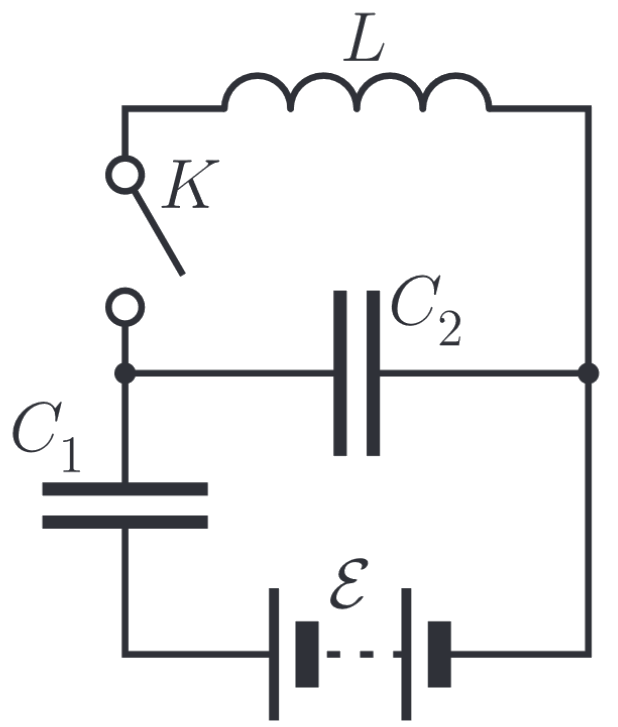
\includegraphics[width=0.35\textwidth]{S5 Figures/S5-151.png}
\end{center}
\end{solution}